\documentclass[11pt]{article}
\usepackage{graphicx} % Required for inserting images
\usepackage[top=2.5cm, bottom=2.5cm, left=2.5cm, right=2.5cm]{geometry}
\usepackage[T1]{fontenc}
\usepackage{hyperref}
\usepackage[utf8]{inputenc}
\usepackage{multirow}
\usepackage{subcaption}
\usepackage{booktabs}
\usepackage{bookmark}
\usepackage{graphicx}
\usepackage{setspace}
\setlength{\parindent}{0in}
\usepackage{physics}
\usepackage{tikz}
\usepackage{tikz-3dplot}
\usepackage[outline]{contour} % glow around text
\usepackage{xcolor}
\usepackage{float}
\usepackage{makeidx}
\usepackage{fancyhdr}
\usepackage{pgfplots}
\usepackage{amsmath}
\pgfplotsset{compat=1.18}
\usepackage{caption}
\usepackage[english,catalan]{babel}
\setlength{\parskip}{11pt}
\usepackage{xcolor}
\usepackage{listings}
\usepackage{marginnote}

\title{\Huge\bfseries Pràctica de simulació: \\ Instal·lació de panells solars fotovoltaics en un habitatge unifamiliar a Catalunya \\ [2ex] \Large}

\author{\begin{tabular}{c}
\textbf{GRUP C3} \\
Isaac Baldi García (1667260)\\
Marcel López Freixes (1668323) \\
Eira Jacas García (1666616) \\
Núria Castillo Ariño (1669145)
\end{tabular}}

\date{07/01/2025}

\begin{document}

\maketitle
\newpage

\tableofcontents
\newpage

\section{Moviment de la Terra al voltant del Sol} \label{sec: seccio_1}
En aquesta secció ens hem proposat simular el moviment de translació de la Terra al voltant del Sol. Per fer-ho hem partit de la Llei de la Gravitació Univeral i hem simplificant el nostre problema de dos cossos a un d'un sol cos sota una força central, $F(r)$.
\begin{equation}
    F(r)=-\frac{GMm}{r^2}
\end{equation}

On G és la constant de grabitació universal, M la massa del Sol i m la massa de la Terra.\footnote{Totes les dades orbitalàries agafades del Jet Propulsion Laboratory de la NASA: \url{https://ssd.jpl.nasa.gov/}}

Per aquest tipus de sistemes i considerant únicament aquesta força central, tenim dues equacions de moviment en el pla polar 
\begin{equation}
    F(r)=m\ddot{r}-mr{\dot{\theta}}^2
    \label{equ_en_r}
\end{equation}
\begin{equation}
    0=\ddot{\theta}m=mr\ddot{\theta}+2m\dot{r}\dot{\theta}
    \label{equ_en_theta}
\end{equation}
i la propietat que el moment angular es conserva
\begin{equation}
    L=mr\dot{\theta}=ctt
    \label{moment_angular}
\end{equation}

Combinant les equacions \eqref{equ_en_r} i \eqref{moment_angular} obtenim una EDO que només depen de r i una EDO que només depen de $\theta$
\begin{equation}
    \frac{\partial\dot{r}}{\partial t}=-GM\frac{1}{r^2}+\frac{L^2}{m^2r^3}
    \label{edor}
\end{equation}
\begin{equation}
    \frac{\partial}{}
    \label{edot}
\end{equation}
Normalitzant aquestes dues equacions i reduint l'ordre de l'equació \eqref{edor} obtenim
\begin{equation}
    \frac{\partial\tilde{v}}{\partial\tilde{t}}=-\frac{1}{\tilde{r}^2}+\frac{1}{\tilde{r}^3}
    \label{1_edo_r}
\end{equation}
\begin{equation}
    \frac{\partial\tilde{r}}{\partial\tilde{t}}=\tilde{v}
    \label{2_edo_r}
\end{equation}
\begin{equation}
    \frac{\partial\tilde{\theta}}{\partial\tilde{t}}=\frac{1}{\tilde{r}^2}
    \label{edo_tetha}
\end{equation}
on les variables normalitzades segueixen $r=\tilde{r}\alpha$, $t=\tilde{t}\frac{\alpha}{\bar{v}}$, $v=\tilde{v}\bar{v}$ i les constants de normalització $\alpha = \frac{\beta}{\kappa}$, $\bar{v}=\frac{\kappa}{(\beta)^{1/2}}$, $\beta=\frac{L^2}{m^2}, \kappa=GM$.

Aquest sistema d'equacions diferencials de primer ordre l'hem resolt numèricament amb el mètode d'Euler i agafant com a condicions de contorn el radi de l'òrbita, la velocitat radial i l'angle al periheli.\footnotemark[\value{footnote}]
Si grafiquem els resultats obtenim
\begin{figure}[h]
    \centering
    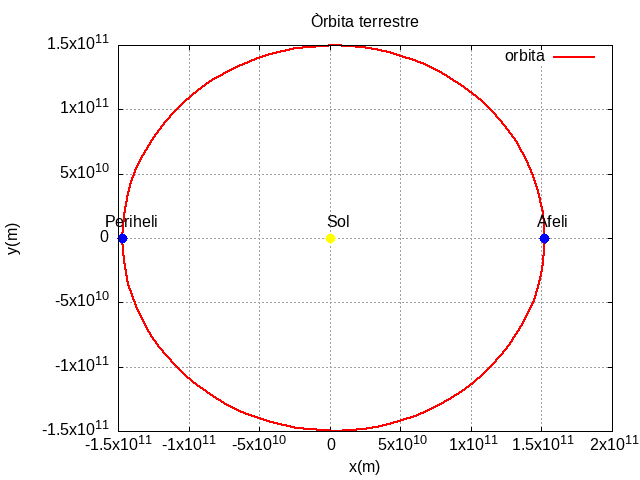
\includegraphics[width=0.5\textwidth]{orbita.png}
    \label{orb_terra}
    \caption{Òrbita Terrestre calculada numèricament}
\end{figure}

El mètode d'Euler és poc exacte però amb una discretització prou fina dona bons resultats. Si calculem l'error acomulat en el radi al completar una Òrbita sencera amb una discretització temporal de $3000$ punts obtenim
\begin{equation}
    Error = \frac{1.47098075136e11-1.47082017410e11}{1.47098075136e11}100\approx0,01\%
\end{equation}
Tot i així a la secció \ref{sec: edos} resoldrem aquest sistema d'EDOs amb altres mètodes per comparar-ne els resultats.


\section{Posició del Sol al cel vist des de l'habitatge} \label{sec: seccio_2}
En aquesta secció ens proposem trobar la posició del Sol des d'un punt determinat de la Terra durant tot l'any.\footnote{\label{nota: habitatge}Per fer els càlculs hem agafat les coordenades d'un habitatge de Sant Cugat del Vallès: 41°28'03.4"N 2°04'28.4"E} Per fer-ho hem parametritzat la posició del sol amb dos angles, l'angle vertical $\nu$ i l'angle horitzontal $\eta$ (\ref{fig: sist_sol}), i hem definit els vectors $\vec{\rho}$, del centre del Sol al punt de la superfície de la Terra, $\vec{r}$, del centre del Sol al punt de la superfície de la Terra, i $\vec{R}$, del centre del Sol al centre de la Terra (\ref{fig: sist_vectors}).
\begin{figure}[hbt]
    \centering
    \begin{subfigure}{0.5\textwidth}
        \centering
        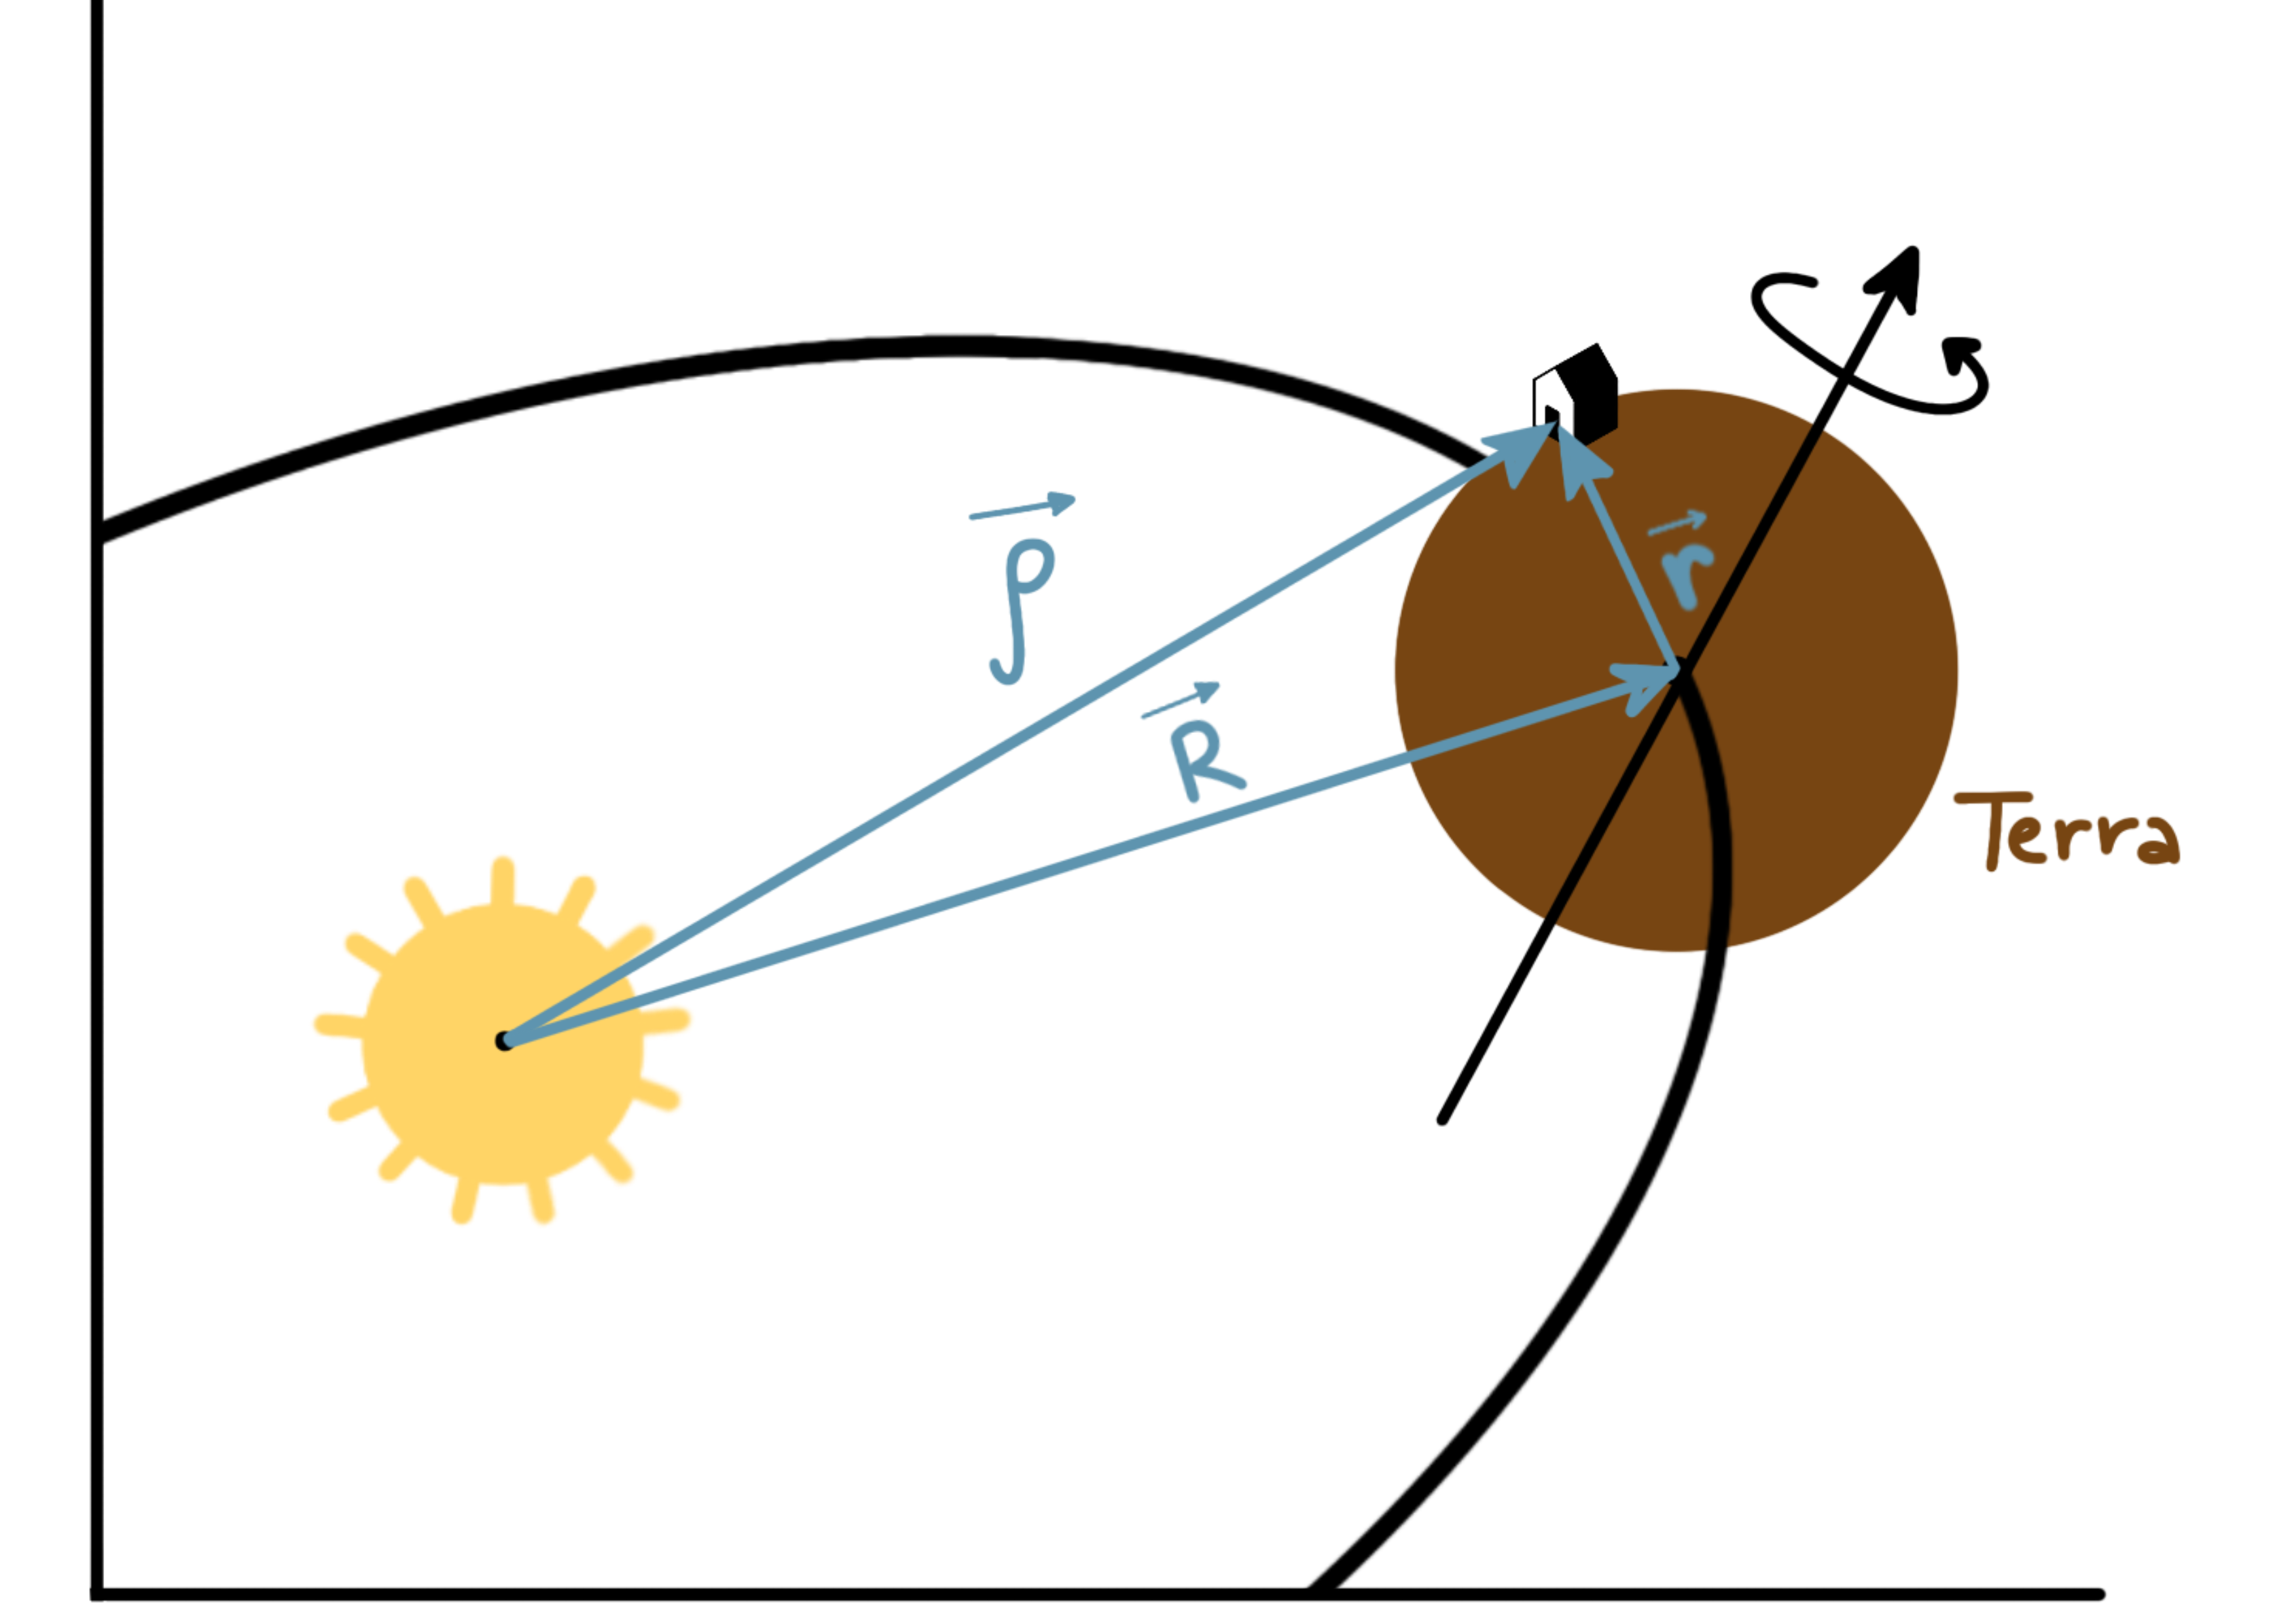
\includegraphics[width=\textwidth]{vectors.PNG}
        \caption{Els vectors que hem definit a la secció \ref{sec: seccio_2}.}
        \label{fig: sist_vectors}
    \end{subfigure}%
    \hspace{0.000001\textwidth}%
    \begin{subfigure}{0.5\textwidth}
        \centering
        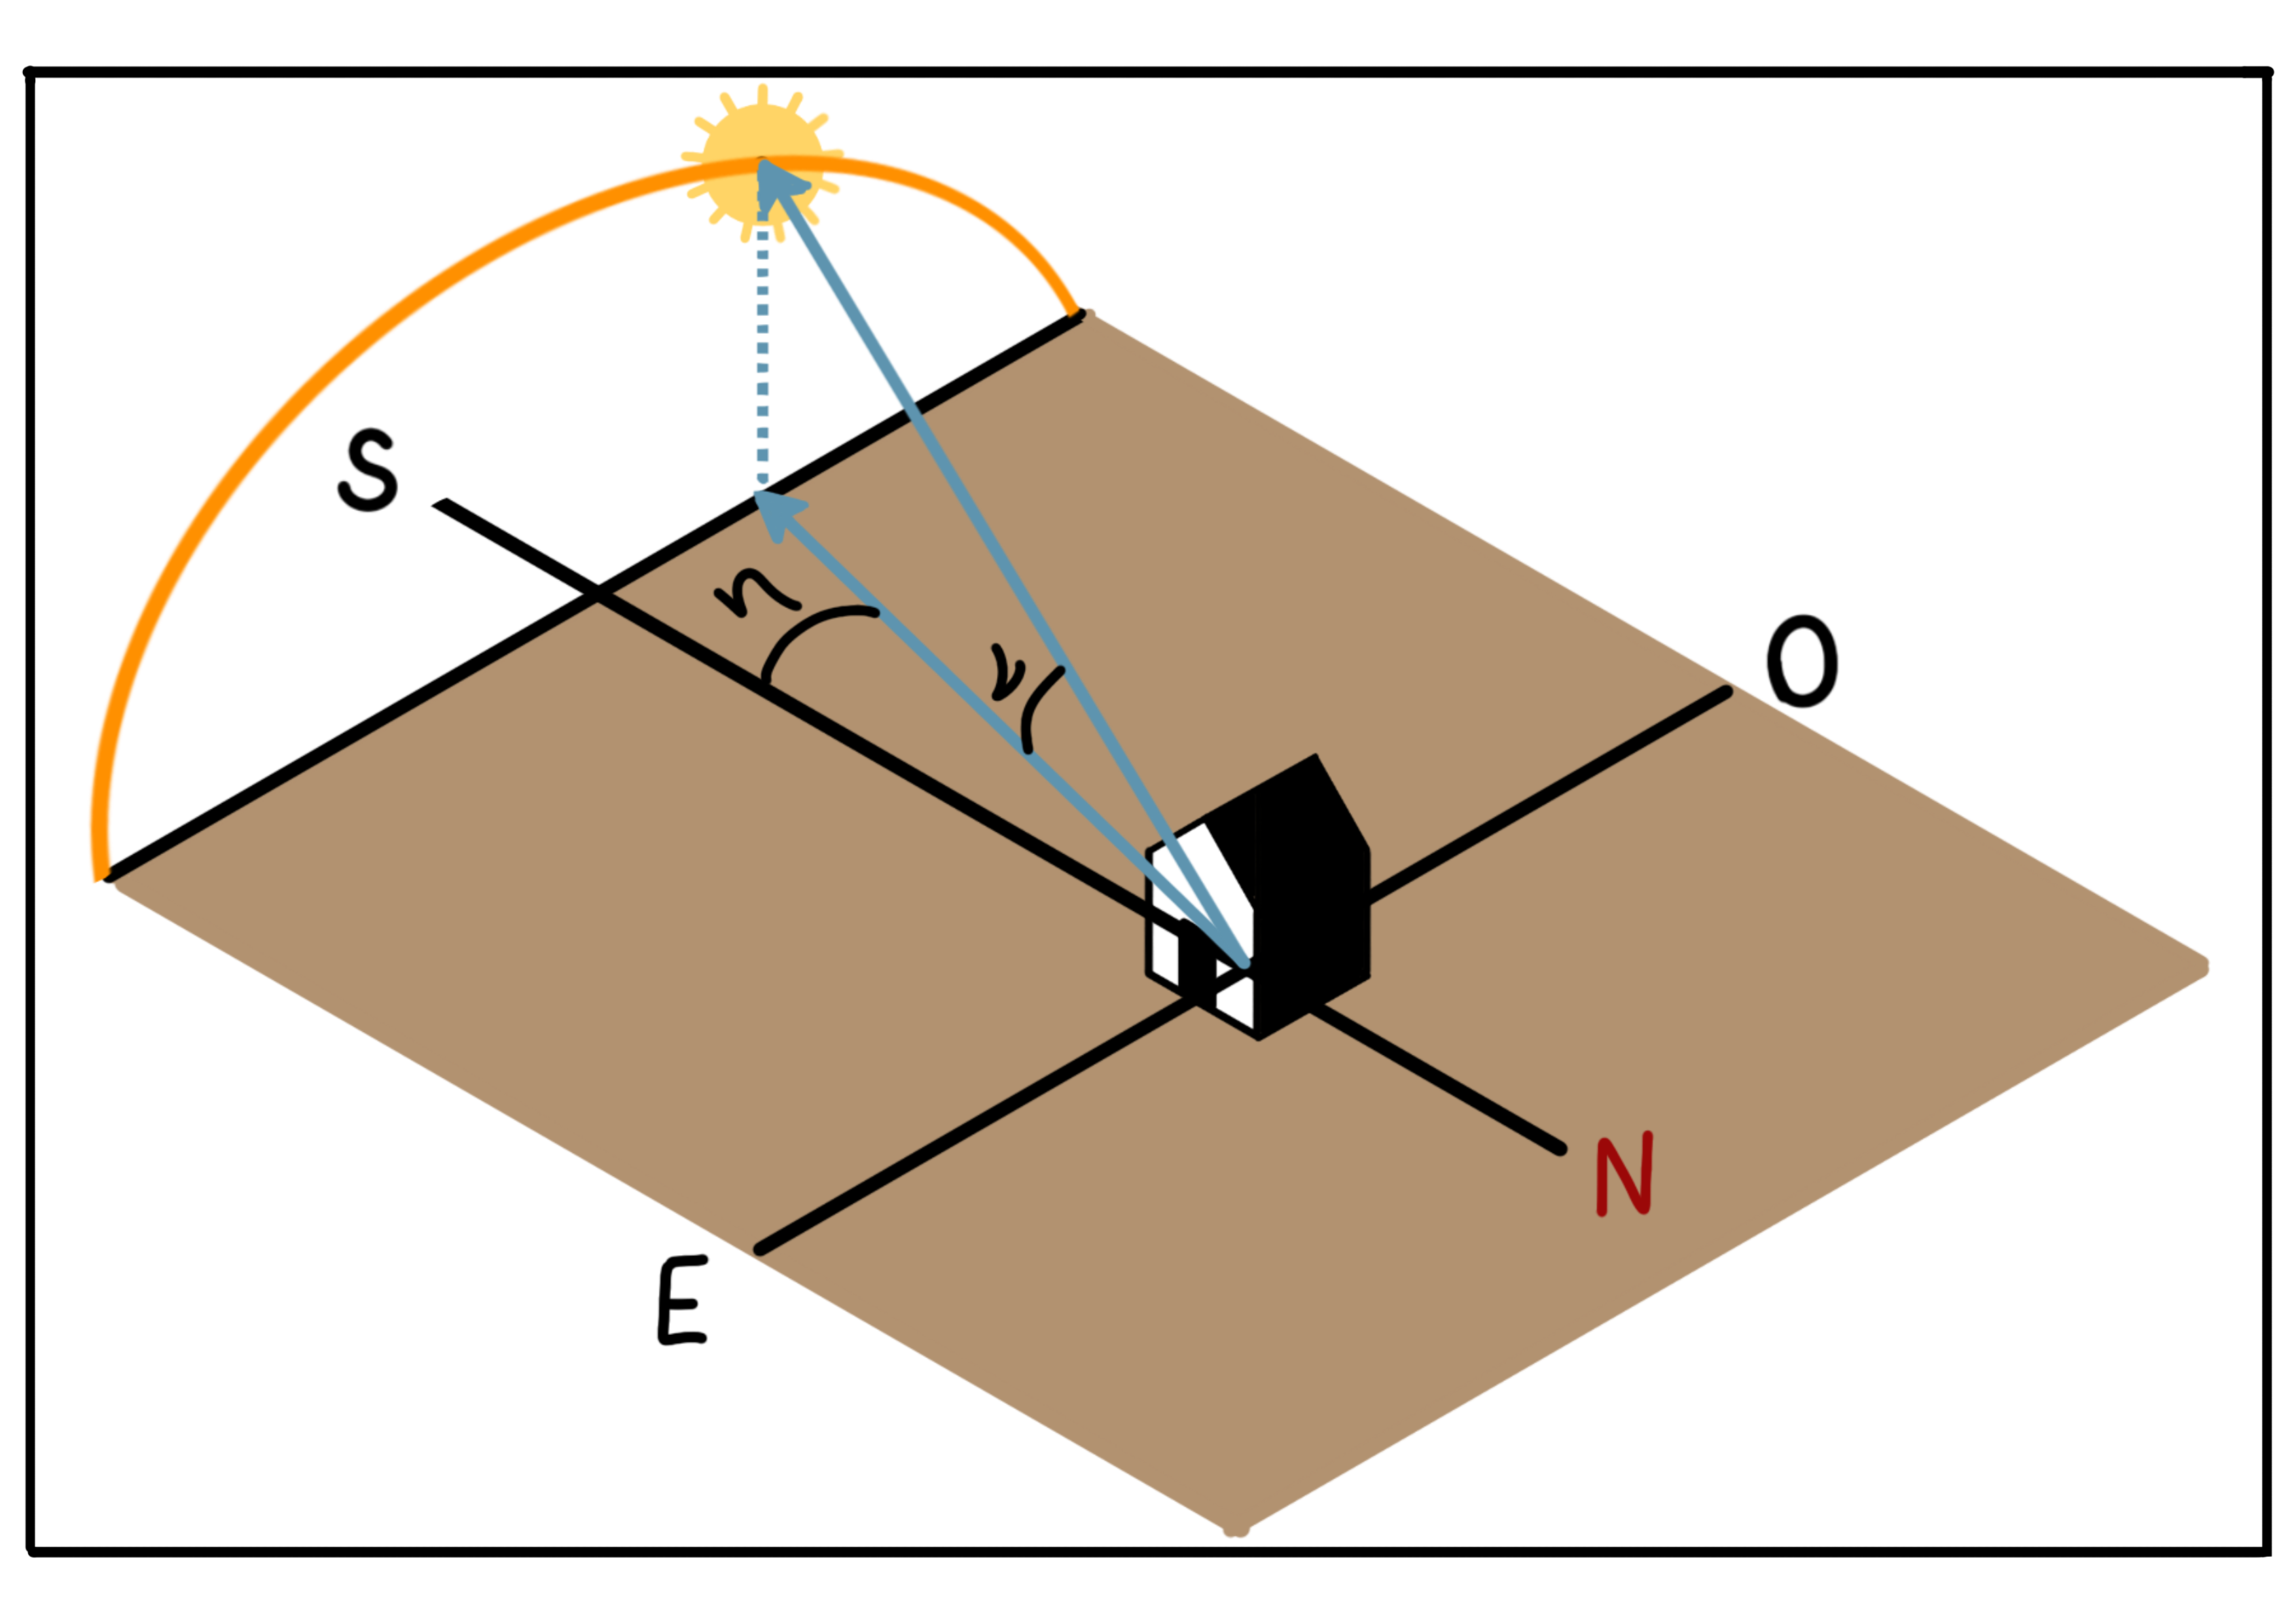
\includegraphics[width=\textwidth]{ang_sol.PNG}
        \caption{Els dos angles que hem usat per a determinar la posició del Sol.}
        \label{fig: sist_sol}
    \end{subfigure}
\end{figure}

També hem definit tres sistemes de referència (figura \ref{fig: sist_ref}) per facilitar els càlculs i trobar els àngles esmentats. Començant al sistema $\Omega$ podem obtenir un vector al sistema $\gamma$ a través de les matrius de rotació de l'annex \ref{annex: matr_rot}. Les relacions entre aquests sistemes són
\begin{itemize}
    \item Sistema $\Omega$: l'eix $z$ està orientat amb l'eix de rotació de la Terra.
    \item Sistema $\beta$: sistema rotat un angle $\beta$ en el pla $zy$ respecte el sistema $\Omega$. $\beta$ és l'angle entre l'eix de rotació de la terra i el vector perpendicular al pla de l'orbita, per tant, ara l'eix $z$ apunta en direcció pendicular al pla de l'òrbita.
    \item Sistema $\gamma$: sistema rotat un angle $\gamma$ en el pla $xy$ respecte el sistema $\beta$. $\gamma$ és l'angle entre $\vec{R}_{periheli}$ i $\vec{R}_{solstici(hivern)}$, per tant, ara la direcció de l'eix $y$ coincideix amb la direcció del periheli.
\end{itemize}
de tal manera que al sistema $\gamma$ tenim l'òrbita de la Terra amb el periheli i l'afeli sobre l'eix y i l'eix de rotació de la Terra orientat per tal que al solstici d'hivern (21 de Desembre) l'angle entre l'eix de rotació de la Terra i la direcció perpendicular al pla de l'òrbita sigui màxim.

Al sistema $\Omega$ el vector $\vec{r}$ és molt fàcil de definir 
\begin{equation}
    \vec{r}_{(t)}=r_T[\cos(\alpha)\cos(wt+\varphi)\hat{e_x}+\cos(\alpha)\sin(wt)+\varphi\hat{e_y}+\sin(\alpha)\hat{e_z}]
    \label{vector_r}
\end{equation}
si tenim la coordenada de latitud del punt de la Terra on volem fer els càlculs, $\alpha$, i el radi de la Terra, $r_T$, i on $w$ és la velocitat angular de rotació de la Terra i $t$ el temps transcorregut al llarg del dia.
Per tal de que aquest vector a $t=0$ comenci a la posició més allunyada del Sol (és a dir que t=0 es correspongui amb la meitat de la nit) hem d'afegir l'angle $\varphi$ a l'angle de rotació. $\varphi$ anirà variant cada dia i és l'angle entre el vector definit a (\ref{vector_r}) i el vector $\vec{R}$ a $t=0$.

El vector $\vec{R}$ ja el tenim calculat de la secció \ref{sec: seccio_1} i el vector $\vec{\rho}$ és simplement
\begin{equation}
    \vec{\rho}= \vec{R}+\vec{r}
\end{equation}
Un cop tenim aquests tres vectors els angles queden definits
\begin{equation}
    \nu=\angle (\vec{r}_{\gamma}, \vec{\rho}_{\gamma}) -\frac{\pi}{2}  
\end{equation}
\begin{equation}
    \eta=\pi - \angle (\vec{R}_{\Omega}, \vec{r}_{\Omega})
\end{equation}
on usem la funció arccosinus per trobar els angles.\footnote{$\angle (\vec{u}, \vec{v})= \arccos\left(\frac{\vec{u} \cdot \vec{v}}{\|\vec{u}\| \|\vec{v}\|}\right)$}


Si calculem aquests angles per una posició concreta a la Terra\footref{nota: habitatge}i pels dies que corresponen als equinocis i als solsticis obtenim el següent gràfic.
\begin{figure}[H]
    \centering
    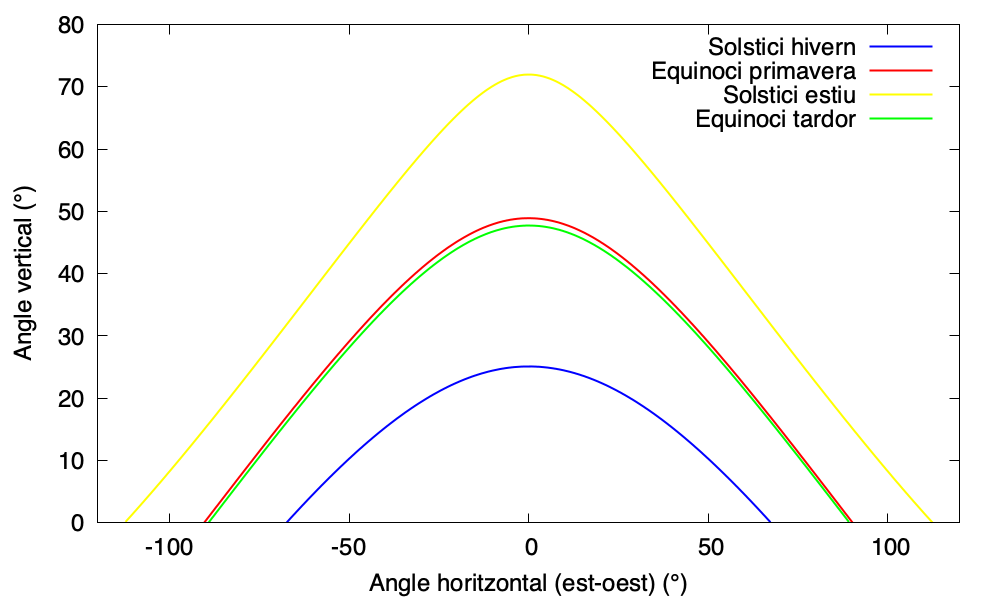
\includegraphics[width=0.5\textwidth]{equinocis.png}
    \label{solsticis}
    \caption{Angles del Sol al llarg d'un dia per diferents moments de l'any a un habitatge de Sant Cugat del Vallès}
\end{figure}

\section{Estudi de l'energia elèctrica}
Suposant que el Sol és un cos negre, segons la llei de Stefan-Boltzmann l'intensitat de radiació emesa pel Sol és $I_S = \sigma_{SB}T_S^4$, on $T_S$ és la temperatura de la superfície del Sol. Així doncs, la potència total emesa ve donada per
\begin{equation}
    P_S = I_SA_S=\sigma_{SB}T_S^4 4 \pi R_S^2
    \label{potencia sol}
\end{equation}
on $A_S$ és l'àrea de la superfície del Sol, el qual hem considerat com una esfera de radi $R_S$.

La intensitat de radiació solar que arriba a un punt a una distància $d$ del Sol $I_d$ és igual la potència $P_S$ dividida entre l'àrea del front d'ona de la radiació, que és una closca esfèrica de radi $d$, considerant que la propagació és radial. Així doncs,
\begin{equation}
    I_d = \frac{P_S}{4\pi d^2}=\frac{1}{d^2}R_S^2\sigma_SB T_S^4
    \label{I_d}
\end{equation}
on a l'última igualtat hem substituit $P_S$ per l'Eq. \eqref{potencia sol}.

Substituint $d$ per la distància del Sol a un determinat punt sobre la superfície terrestre, $\rho$, a l'Eq. \eqref{I_d}, podem calcular la intensitat de radiació que hi incideix. Per considerar l’efecte de l’albedo terrestre, cal multiplicar aquesta intensitat per un factor $\alpha$, que representa la fracció de radiació absorbida per la Terra. Així doncs, la intensitat de l'ona incident és $I_0=\alpha I_{\rho}$.

Degut a la inclinació de la placa, la intensitat efectiva que rebrà serà igual a $I_0 \cos{\theta}$, on $\theta$ és l'angle d'incidència de la radiació, és a dir, l'angle entre la direcció de la llum incident i la normal a la superfície. Per tant, la potència que arriba a la placa ve donada per
\begin{equation}
    P_{inc} = A \alpha I_{\rho} \cos{\theta}
    \label{P_inc placa}
\end{equation}
on $A$ és l'àrea de la placa i hem substituit $I_0$.

Finalment, la potència elèctrica generada per la placa, $P$, és igual a $P_{inc}$ multiplicada per un factor $r$, el rendiment de la placa. Així doncs, substituint l'Eq. \eqref{I_d} en l'Eq. \eqref{P_inc placa}, obtenim
\begin{equation}
    P = r \alpha \frac{1}{\rho^2}R_S^2\sigma_{SB}T_S^4A_p \cos{\theta}
    \label{potencia placa}
\end{equation}
Els valors numèrics dels paràmetres en aquesta equació es troben a la secció 

La normalització de les variables de l'equació anterior ve donada per
\begin{equation}
    \hat{\rho}=\frac{\rho}{\rho_0} \ , \quad
    \hat{P}=\frac{P}{P_0}
\end{equation}
on hem definit els paràmetres característics $\rho_0$ com la distància ???? i $P_0$ com
\begin{equation}
    P_0 = r \alpha \frac{1}{d_0^2}R_S^2\sigma_{SB}T_S^4A_p
    \label{potencia}
\end{equation}
En quant a la variable $\theta$, al tractar-se d'un angle ja és adimensional, i per tant la donem per normalitzada.

Així doncs, segons aquesta normalització l'Eq. \eqref{potencia placa} esdevé
\begin{equation}
    \hat{P} = \frac{\cos{\theta}}{\hat{\rho}^2} \ .
    \label{pot norm}
\end{equation}
Per a determinar $\cos{\theta}$, utilitzem la següent expressió:
\begin{equation}
    \cos \theta = \cos \theta_z \cos \beta + \sin \theta_z \sin \beta \cos (\gamma_s - \gamma) \ .
    \label{cos theta}
\end{equation}
Les definicions dels angles i la demostració d'aquesta equació es dona a la secció \ref{sec: cos theta} de l'annex.

És important destacar que si $\theta_z$ i/o $\theta$ no es troben dins del rang $[-\pi/2,\pi/2]$ imposem que la potència sigui nul·la. En el cas de $\theta_z$ ho imposem pel fet que per a angles fora d'aquest interval el Sol es troba per sota de l'horitzó, cosa que implica que la Terra bloqueja la radiació solar i, per tant, no arriba llum a la placa. De manera similar, el fet que $\theta$ prengui valors fora d'aquest interval significa que el Sol està situat darrere la placa, és a dir, que és la pròpia placa la que bloqueja la llum solar.


\section{Energia elèctrica produïda per la placa}

Amb la potència elèctrica generada per la placa cada minut de l'any ens disposem a calcular l'energia elèctrica produïda per aquesta. La potència és la derivada temporal de l'energia, per tant, podem trobar l'energia elèctrica produïda per la placa durant una certa quantitat de temps integrant numèricament la potència respecte el temps. Per fer-ho, hem optat pel mètode d'integració numèrica de Simpson $\frac{1}{3}$. Presentem l'energia produïda cada dia de l'any a la Fig. \ref{fig: energies} .


\begin{figure}[h]
    \centering
    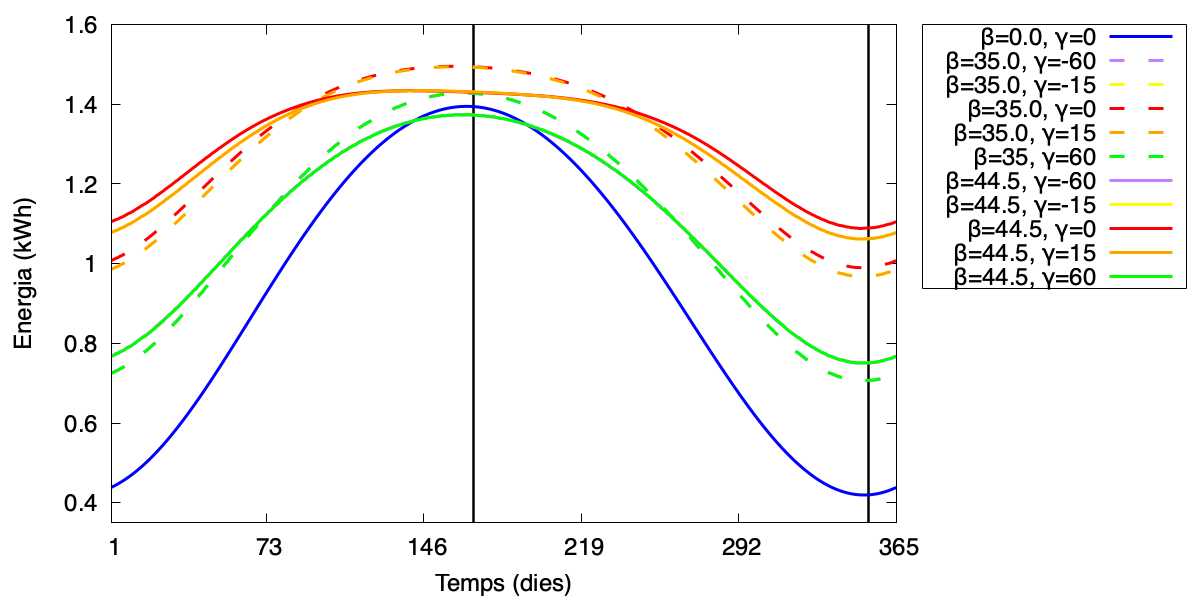
\includegraphics[width=0.75\linewidth]{energia.png}
    \caption{Energia elèctrica produïda per la placa cada dia de l'any.}
    \label{fig: energies}
\end{figure}

Les linies negres indiquen els solsticis d'estiu i hivern on l'energia elèctrica produïda arriba en tots els casos a un màxim i un mínim, respectivament.

\section{Optimització dels angles de la placa}

Hem plantejat el problema des del punt de vista de maximitzar la producció d'energia total al llarg d'un any mantenint els angles $\beta$ i $\gamma$ de la placa constants durant tot l'any. Per fer-ho, hem utilitzat que l'energia total produïda en un any la podem escriure com
\[
E_T(\beta, \gamma) = \cos \beta \int r I_{\text{abs}} A_{t} \cos \theta_{z} \, dt
+ \sin \beta \cos \gamma \int r I_{\text{abs}} A_{t} \sin \theta_{z} \cos \gamma \, dt
+ \sin \beta \sin \gamma \int r I_{\text{abs}} A_{t} \sin \theta_{z} \sin \gamma \, dt=
\]
\[
= a\cos \beta
+ b\sin \beta \cos \gamma
+ c\sin \beta \sin \gamma
\]
Igualant el gradent a 0, trobem que
\[
\left.
\begin{aligned}
-a\sin \beta + b\cos \beta \cos \gamma + c\cos \beta \sin \gamma = 0 \\
-b\sin \beta \sin \gamma + c\sin \beta \cos \gamma = 0
\end{aligned}
\right\}
\]
La solució corresponent per beta i gamma és
\[
\gamma = \arctan\left(\frac{c}{b}\right), \quad \beta = \arctan\left(\frac{b \cos(\gamma) + c \sin(\gamma)}{a}\right)
\]
on hem descartat la solució corresponent a $\beta=n\pi$ per no ser un màxim.

Calculant numèricament les integrals $a$, $b$ i $c$ per Simpson 1/3 sota la condició de que $-\frac{\pi}{2} \leq \theta_z \leq \frac{\pi}{2}$ (en cas contrari l'integrand l'hem anul·lat), hem obtingut uns angles òptims arrodonint a la primera xifra decimal de $\gamma=0^\circ$ i $\beta=44,5^\circ$, l'energia produïda dia a dia durant tot l'any corresponent a aquests angles pot trobar-se a la Fig. \ref{fig: energies}. 

Pel que fa al valor de gamma obtingut, era d'esperar que aquest fos de $0^\circ$, ja que a l'hemisferi nord el Sol arriba al seu punt més alt al cel (i, per tant, al punt on els raigs incideixen més perpendicularment a una superfície donada) en direcció sud durant el dia, per tant, aquesta orientació maximitza les hores d'exposició directa al Sol. Per altra banda, l'angle $\beta$ obtingut entra dins l'esperat si tenim en compte que s'assembla a la latitud considerada en el nostre cas (uns $41,5^\circ$) que teòricament serà l'inclinació òptima, ja que ens permetrà captar de manera més perpendicular els raigs de sol (una manera de pensar-ho és que a l'equador aquesta inclinació seria 0 perquè el sol ens passaria per sobre del cap, a mesura que ens allunyèssim de l'ecuador, o incrementèssim la nostra latitud, més hauriem d'inclinar la placa). Per altra banda, a la Fig. \ref{fig: energies} podem observar que a l'estiu un angle d'inclinació de $35^\circ$, per exemple, produeix més energia que un de $44,5^\circ$, ara bé, com hem dit, nosaltres hem maximitzat la producció total durant l'any. Això, però, suggereix que durant diferents èpoques de l'any podriem modificar l'inclinació de la placa per així maximitzar la seva producció.




\section{Resolució de l'EDO per diversos mètodes numèrics}\label{sec: edosRK}
Per a resoldre l'EDO de l'òrbita terrestre hem utilitzat el mètode d'Euler, però sabem que hi ha mètodes numèrics més potents que aquest. Per axò hem volgut comparar els resultats.

Els mètodes emprats per a resoldre l'equació \eqref{equ_en_r} han estat el Runge-Kutta d'ordre 2 i el Runge-Kutta d'ordre 4, amb la mateixa discretització temporal en els 3 mètodes numèrics.

\begin{figure}[hbt!]
    \centering
    \begin{subfigure}{0.5\textwidth}
        \centering
        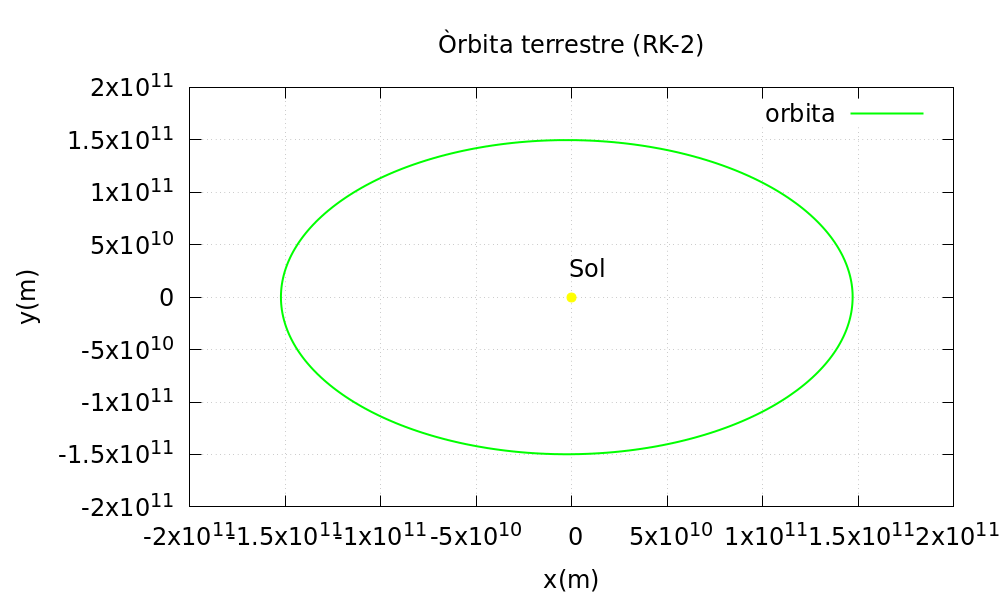
\includegraphics[width=\textwidth]{orbitaRK2.PNG}
        \caption{Òrbita terrestre per Runge-Kutta d'ordre 2}
        \label{fig: orbitaRK2}
    \end{subfigure}%
    \vspace{0.01\textwidth}%
    \begin{subfigure}{0.5\textwidth}
        \centering
        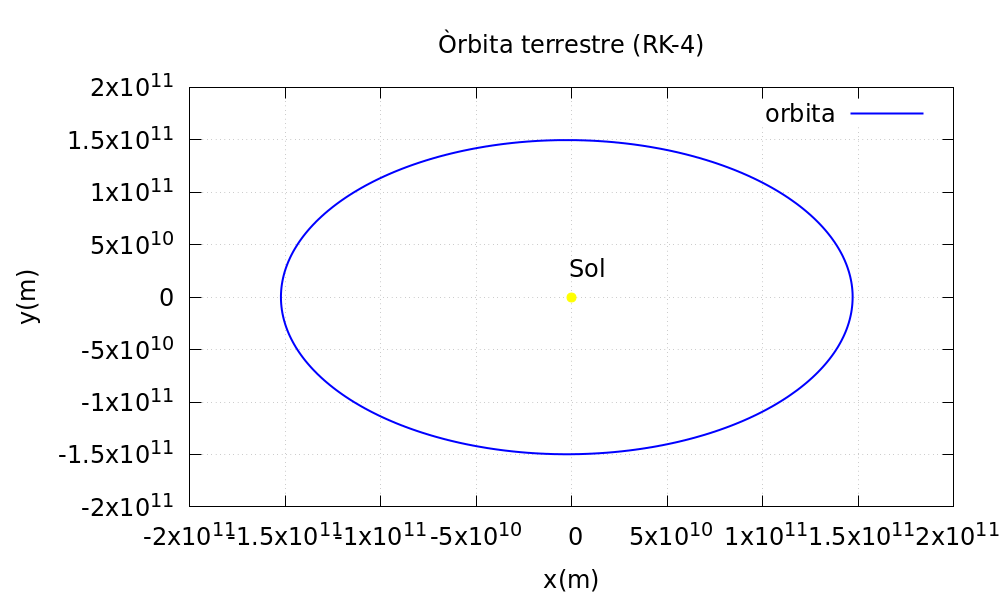
\includegraphics[width=\textwidth]{orbitaRK4.PNG}
        \caption{Òrbita terrestre per Runge-Kutta d'ordre 4}
        \label{fig: orbitaRK4}
    \end{subfigure}
    \vspace{0.01\textwidth}%
    \begin{subfigure}{0.5\textwidth}
        \centering
        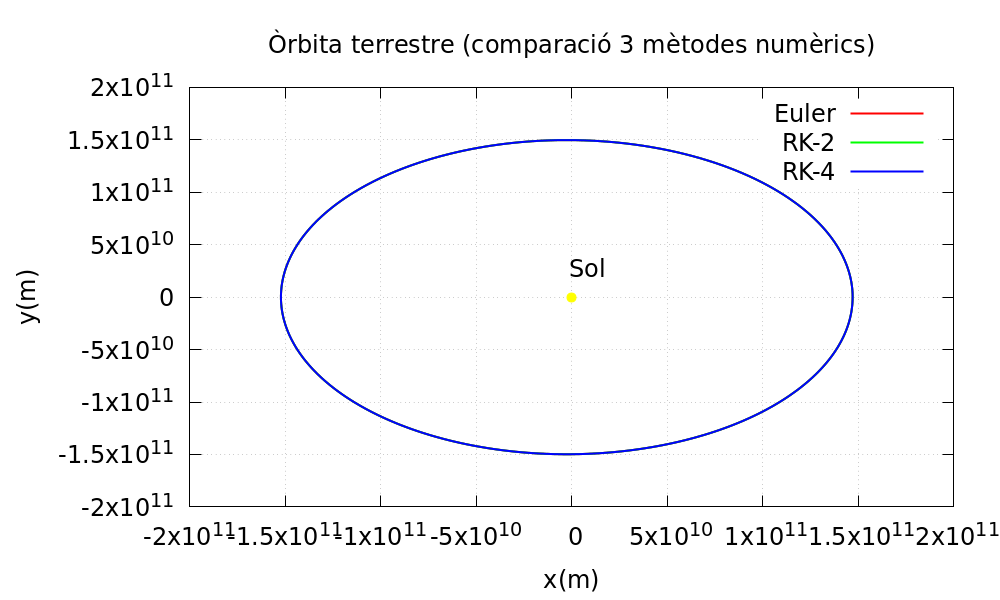
\includegraphics[width=\textwidth]{orbita3met.PNG}
        \caption{Òrbites terrestres per 3 mètodes numèrics}
        \label{fig: orbita3met}
    \end{subfigure}
\end{figure}

\section*{Annex}
\appendix

\section{Matrius de canvi de sistema de referència}\label{annex: matr_rot}
\begin{equation}
    \mathbf{R}_{\beta}=
    \begin{pmatrix}
      1 & 0 & 0   \\
      0 & \cos\beta& -sin\beta \\
      0 & sin\beta & cos\beta \\
    \end{pmatrix}
\end{equation}  

\begin{equation}
    \mathbf{R}_{\gamma}=
    \begin{pmatrix}
       \cos\beta& -sin\beta& 0 \\
       \sin\beta & cos\beta &0\\
      0 & 0 & 1  \\
    \end{pmatrix}
\end{equation}  


\section{Angles i vectors apartat 2}
\begin{figure}[hbt]
    \centering
    \begin{subfigure}{0.5\textwidth}
        \centering
        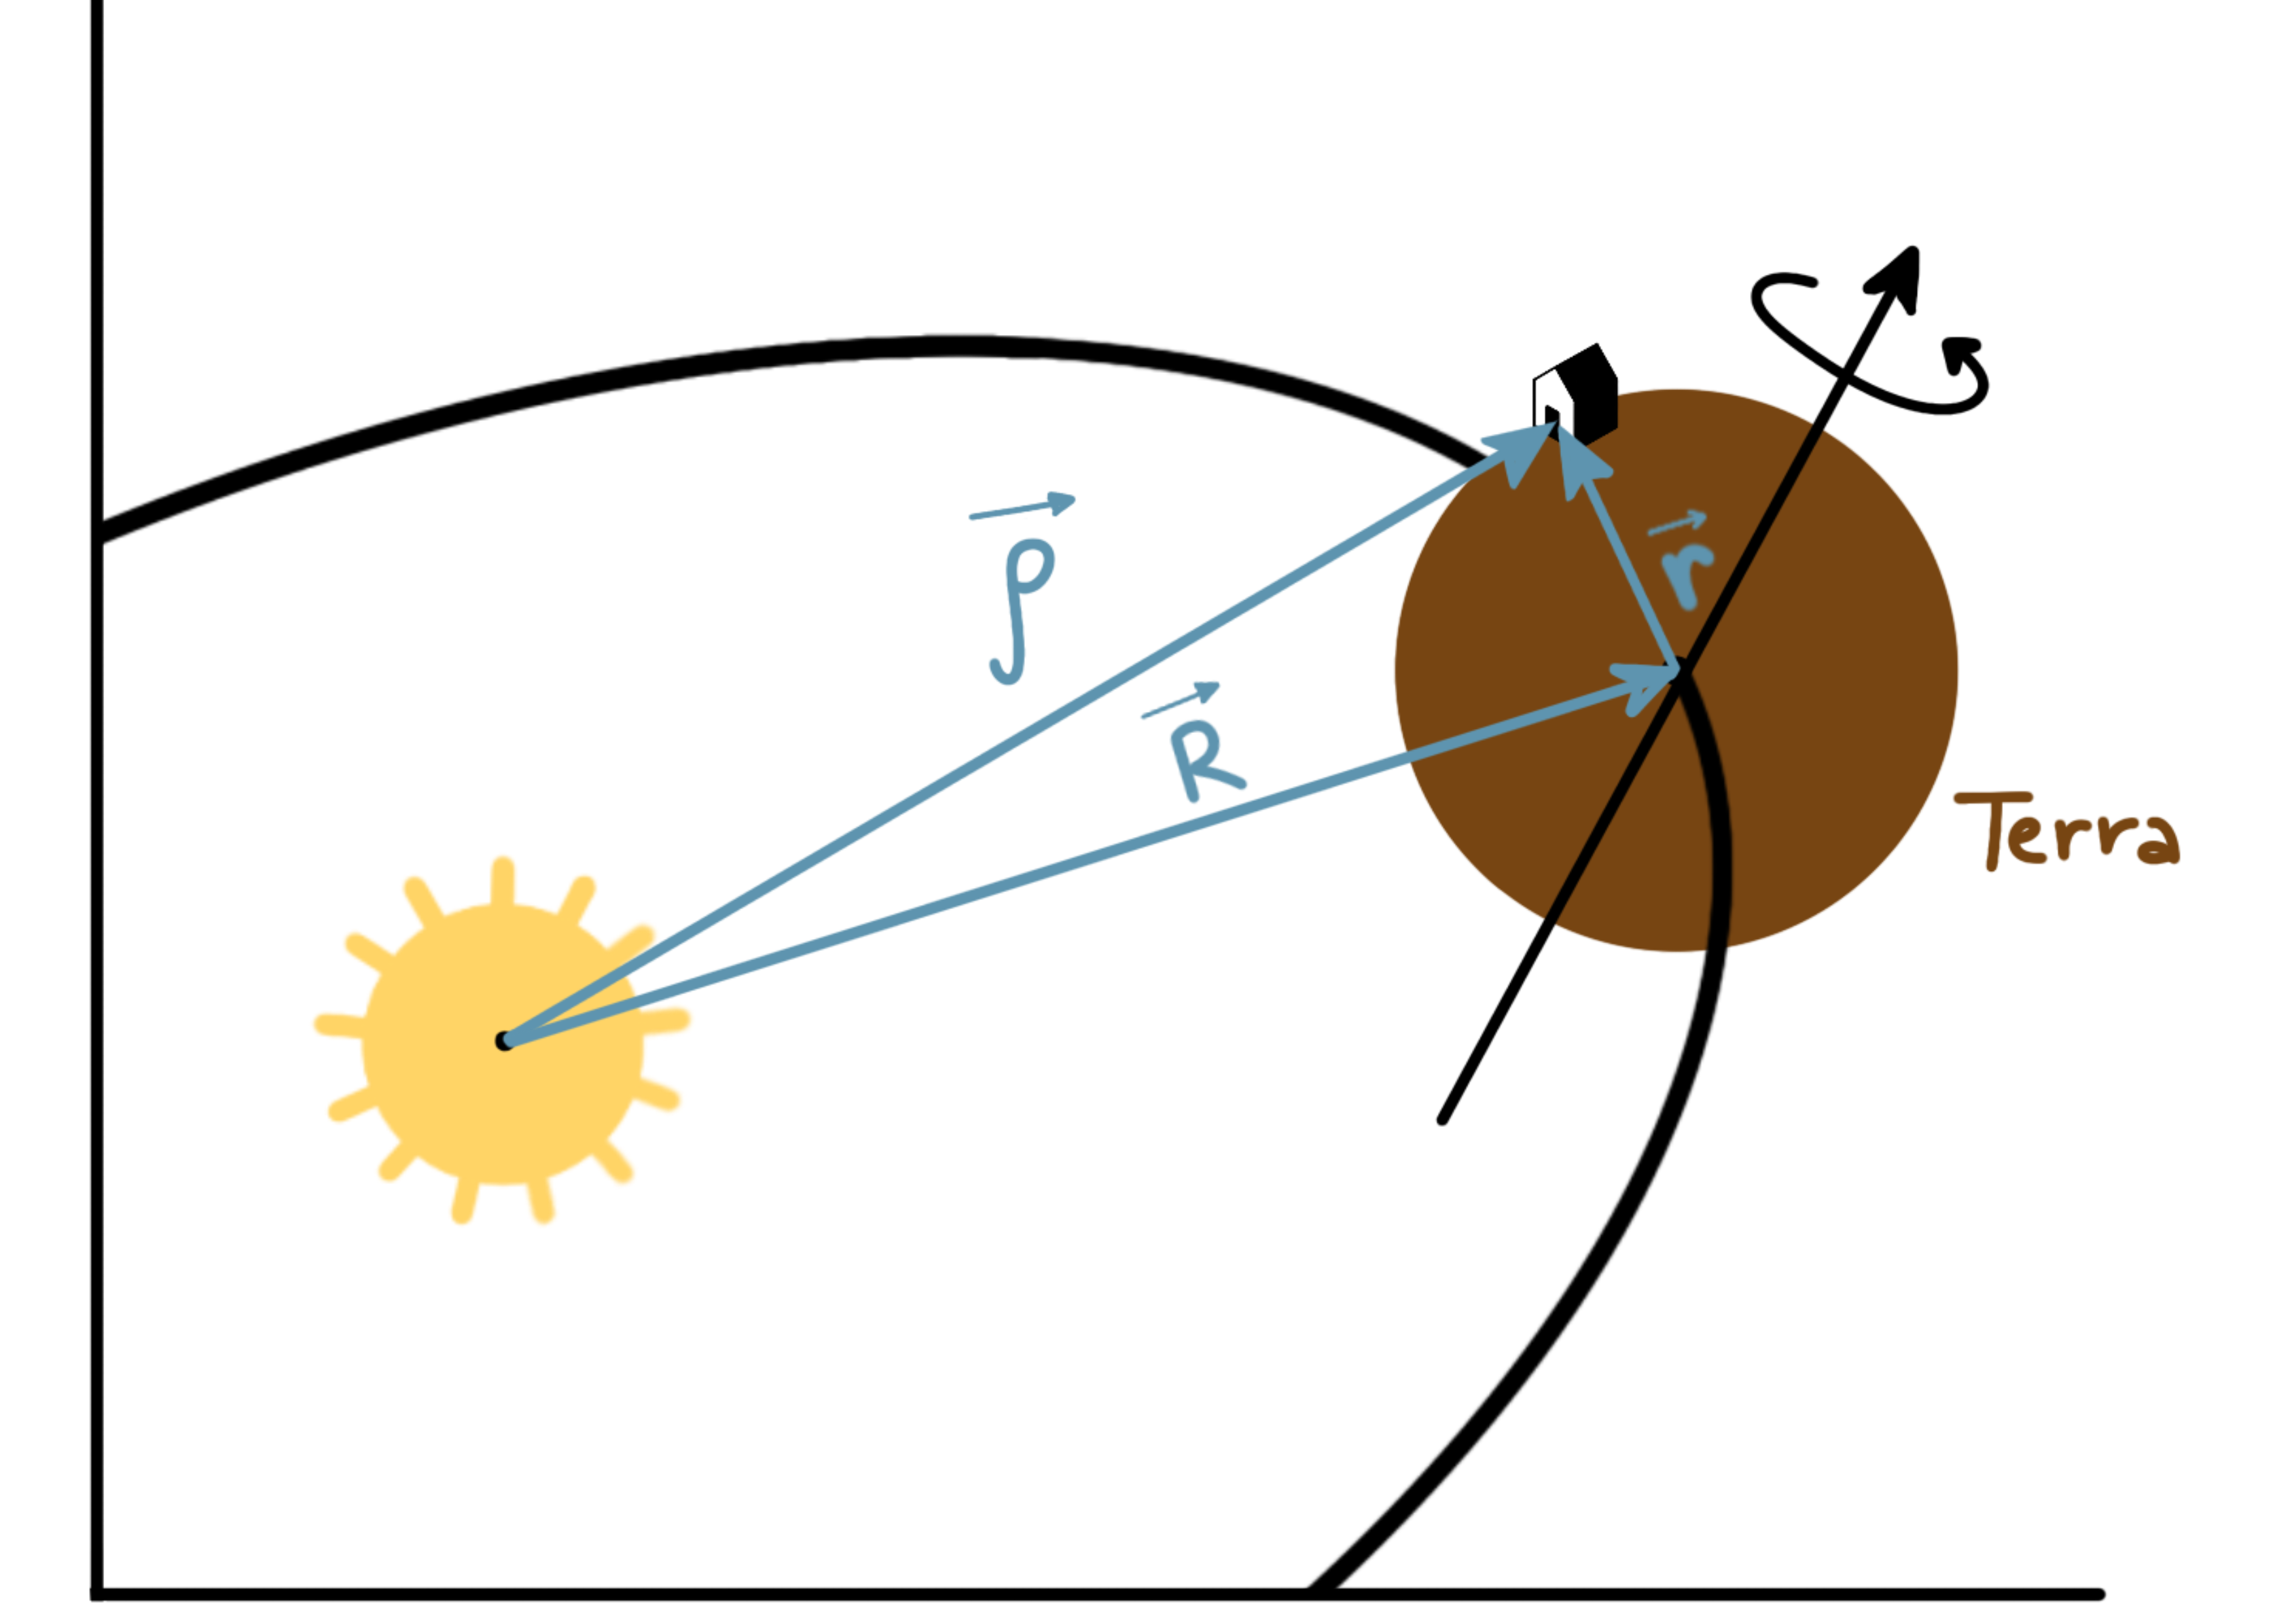
\includegraphics[width=\textwidth]{vectors.PNG}
        \caption{Els vectors que hem definit a la secció \ref{sec: seccio_2}.}
        \label{fig: sist_vectors}
    \end{subfigure}%
    \hspace{0.000001\textwidth}%
    \begin{subfigure}{0.5\textwidth}
        \centering
        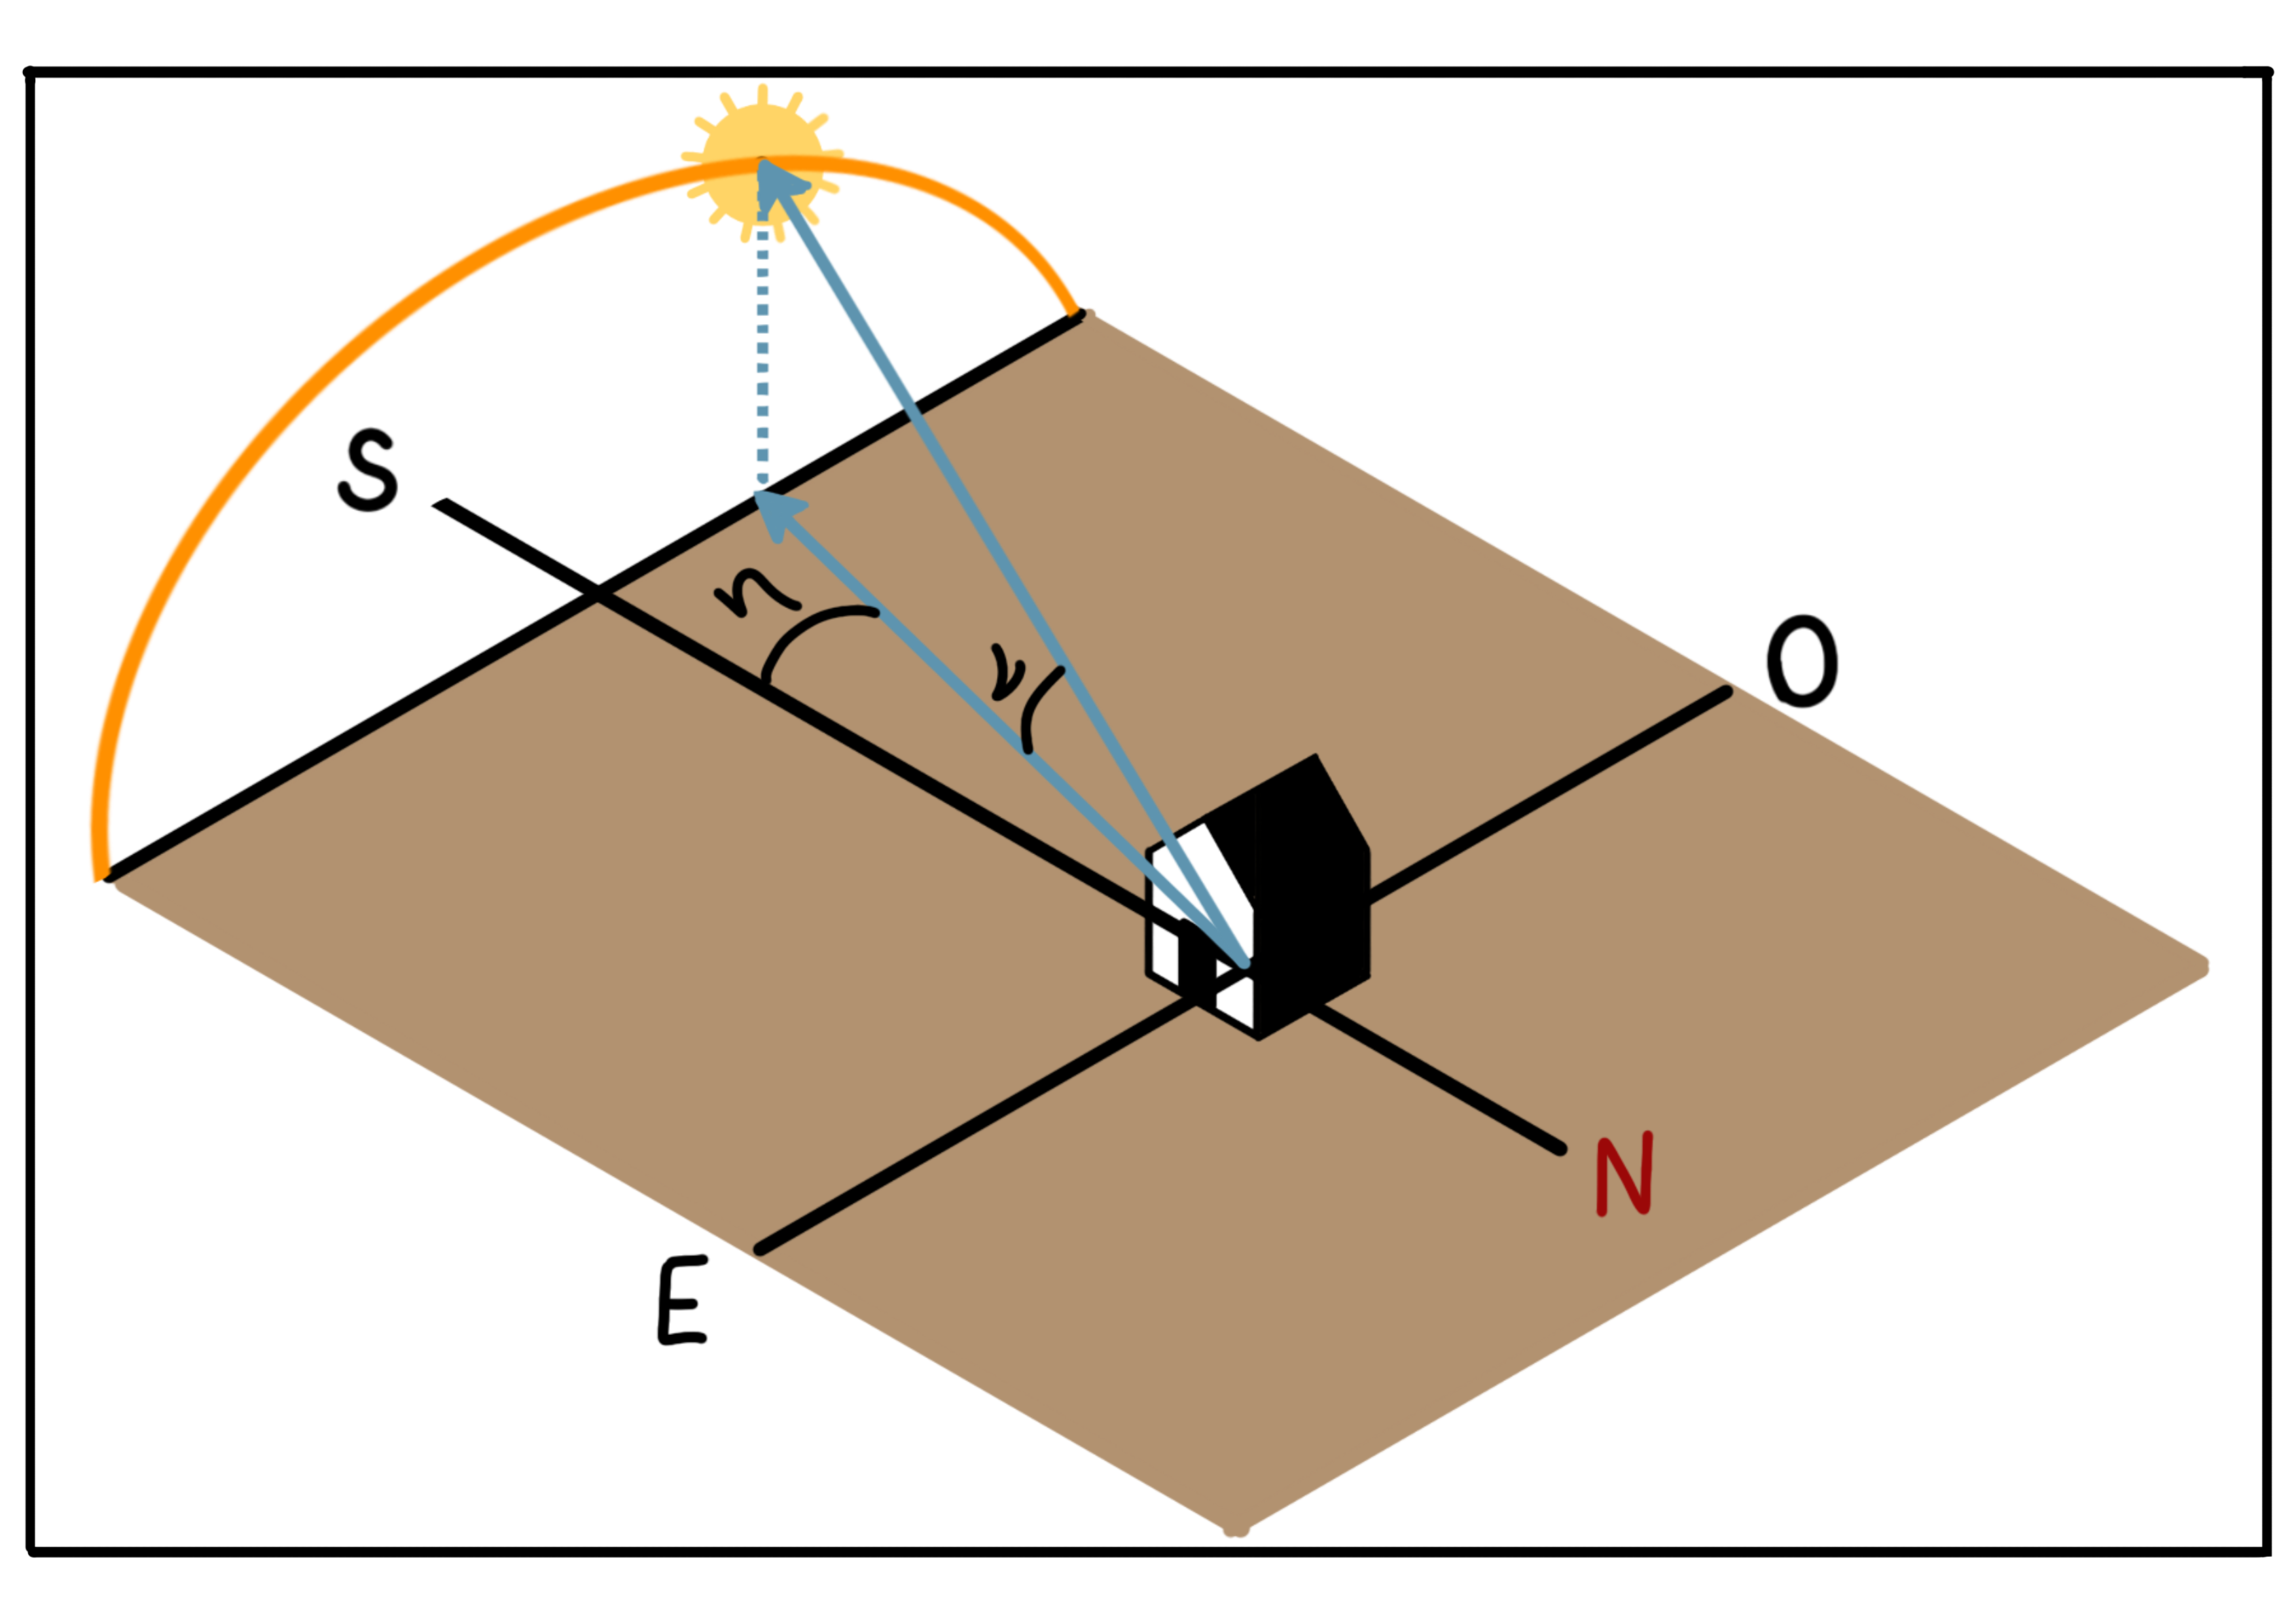
\includegraphics[width=\textwidth]{ang_sol.PNG}
        \caption{Els dos angles que hem usat per a determinar la posició del Sol.}
        \label{fig: sist_sol}
    \end{subfigure}
\end{figure}

\begin{figure}[hbt]
    \centering
    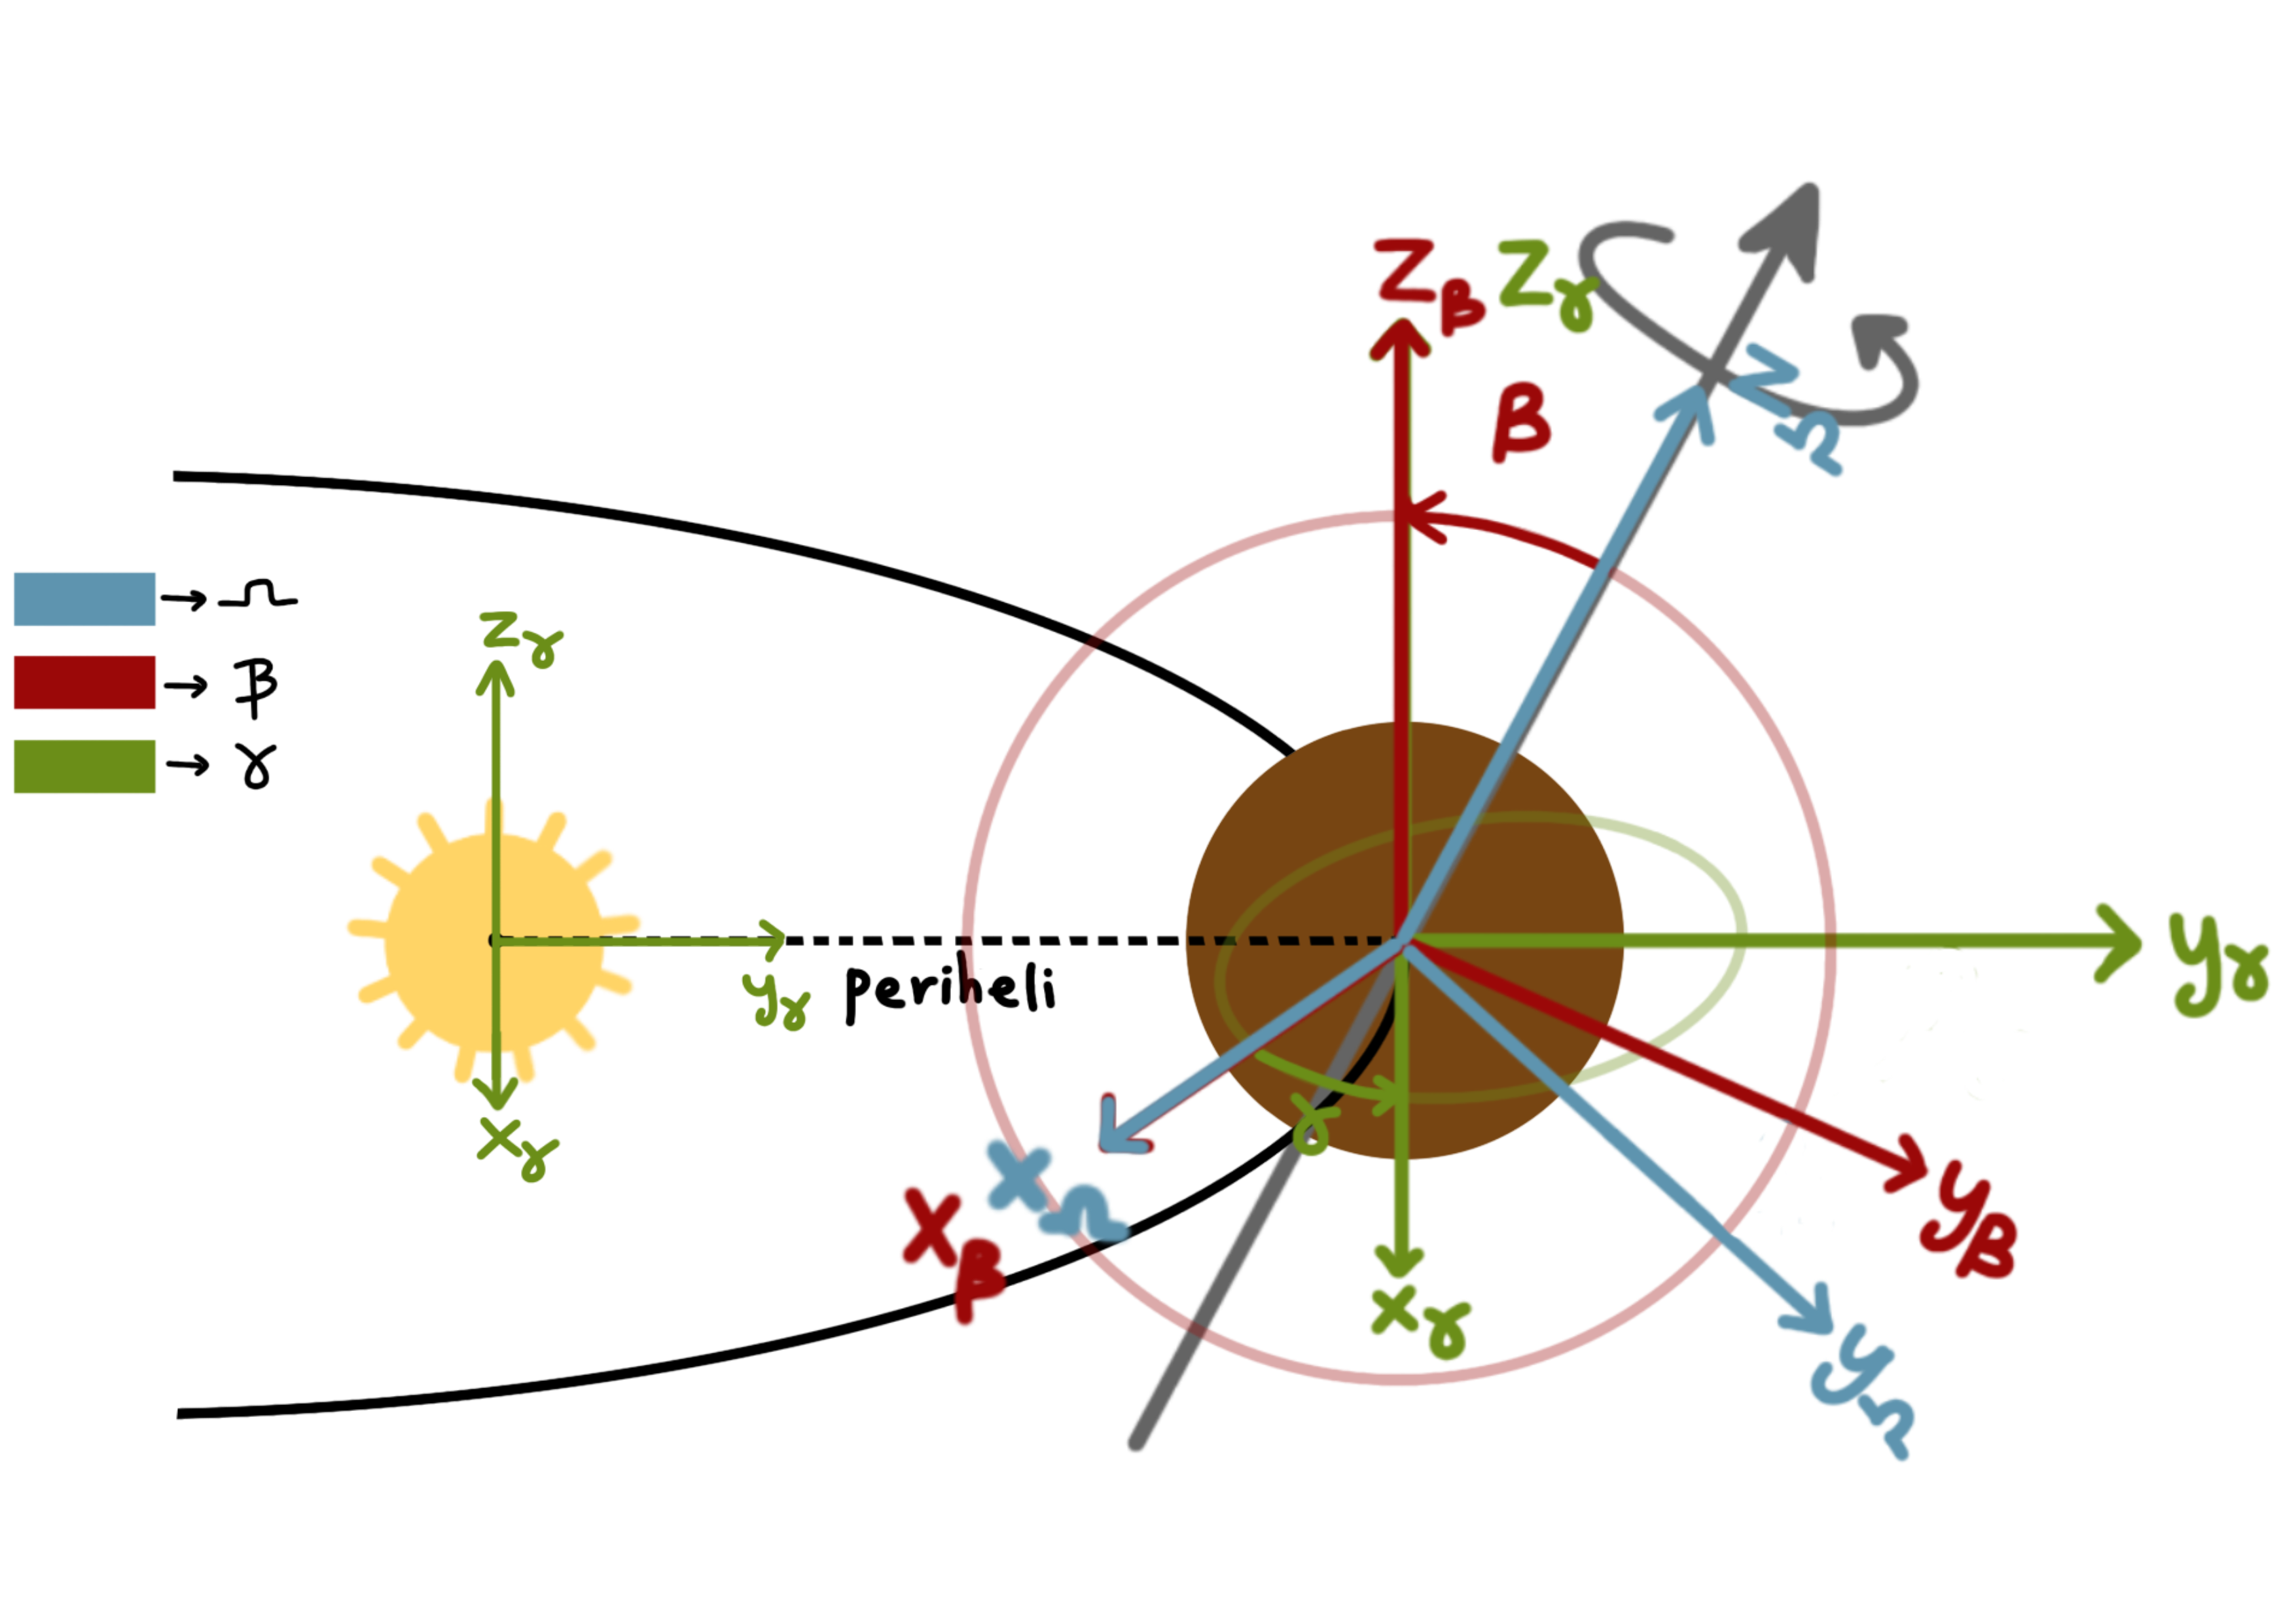
\includegraphics[width=0.5\textwidth]{sist_ref.PNG}
    \caption{Diferents sistemes de referència de la secció \ref{sec: seccio_2}.}
    \label{fig: sist_ref}
\end{figure}
\end{document}